\documentclass[11pt]{amsart}
\usepackage[margin=1.1in]{geometry}
\usepackage{amsmath,amssymb,amsthm}
\usepackage{graphicx}
\usepackage{booktabs}
\usepackage{enumitem}
\usepackage[hidelinks]{hyperref}
\usepackage{url}

\newtheorem{theorem}{Theorem}
\newtheorem{lemma}{Lemma}
\newtheorem{proposition}{Proposition}
\newtheorem{corollary}{Corollary}
\theoremstyle{definition}
\newtheorem{definition}{Definition}
\theoremstyle{remark}
\newtheorem{remark}{Remark}

\newcommand{\R}{\mathbb{R}}
\newcommand{\Z}{\mathbb{Z}}
\newcommand{\Q}{\mathbb{Q}}
\newcommand{\e}{\mathbf{e}}
\newcommand{\vu}{\mathbf{u}}
\newcommand{\va}{\mathbf{a}}
\newcommand{\vb}{\mathbf{b}}
\newcommand{\vv}{\mathbf{v}}
\newcommand{\nus}{\nu_{100}}
\newcommand{\norm}[1]{\lVert#1\rVert}

\title[The bridged cross-polytope framework]{The bridged cross-polytope framework: unit-spring elastic constants in every dimension and an exact motion from the CaB$_6$ boron net to face-centred cubic packing}

\author{Ahraz Arifuddin}
\address{Aska Digital}

\date{13 October 2026. Version 2.}

\begin{document}

\begin{abstract}
Place a ball at the incentre of each of the $2n$ pyramids that join the centre of an $n$-cube to its facets. The balls form regular cross-polytopes, one per cell of the cubic lattice, and neighbouring cross-polytopes touch through one bar per axis. In three dimensions this is the boron net of CaB$_6$ (RCSR \textsf{cab}). We prove two results about this bridged cross-polytope framework. First, with unit springs on all bars, every shear modulus vanishes, $C_{11}/C_{12}=(n-1)^2$, and the Poisson ratio for uniaxial stress along a cube axis is $\nus=1/(n^2-n-1)$, for every $n\ge3$. Second, in three dimensions there is an explicit motion, rational in a parameter $s$ over $\Q(\sqrt2)$, that keeps every bar length, keeps the octahedra in a fixed orientation while the lattice deforms, raises the packing fraction strictly from $0.2233$ to $\pi/\sqrt{18}$, and ends in face-centred cubic packing. No two balls overlap at any parameter value; we give a written proof that uses the monoclinic symmetry of the path and a bound on the deformed lattice, and an independent exact certificate. The zero-mode and self-stress counts $n(n-1)/2$ and $n(n-3)/2$ per cell, on which the elastic proof rests, are recorded as lemmas: the same periodic graph appears in Borcea and Streinu, and the counts follow from standard periodic-rigidity arguments. As secondary results we record a radius-ratio identity for the incentre construction, with its exact hypotheses and counterexamples, and the maximal hard-sphere packing fraction $(\pi/6)(30\sqrt2-41)$ of the CaB$_6$ structure type. Every number is reproduced by scripts in a public repository.
\end{abstract}

\maketitle

\noindent\emph{Version 2. Supersedes v1 (doi:\href{https://doi.org/10.5281/zenodo.23322080}{10.5281/zenodo.23322080}), whose novelty claims for the rigidity counts are corrected here.}

\section{Introduction}

Draw a square and its diagonals, mark the incentre of each of the four triangles, and repeat the square over the plane. A ball of the inradius at each incentre touches its two neighbours across the diagonals and one ball of the next square across the shared side. The same holds in every dimension. If an $n$-cube of side $2$ is cut into the $2n$ pyramids that join its centre to its facets, the incentre of each pyramid lies on an axis at distance $c=2-\sqrt2$ from the centre and has inradius $R=\sqrt2-1$. Balls of radius $R$ at these $2n$ points touch along all edges of the cross-polytope they span and across every facet of the cubic tiling (Fig.~\ref{fig:construction}). The bars between touching balls form a periodic framework: regular cross-polytopes, one per cell, joined by one bridge per axis. We call it the \emph{bridged cross-polytope framework}.

\emph{What is known.} The triangles of the drawing are fundamental domains of the $[4,4]$ reflection group, and the orbit of the incentre is the vertex set of the truncated square tiling 4.8.8; in dimension $n$ the incentre is the Wythoff point of $t_{0,1}\{4,3^{n-2},4\}$ \cite{Coxeter1973,ConwayBurgielGS2008,GrunbaumShephard1987}. In three dimensions the vertex set, with equal bonds, is the boron net of CaB$_6$ in the model of Pauling and Weinbaum \cite{PaulingWeinbaum1934}, the RCSR net \textsf{cab} \cite{OKeeffe2008RCSR,RCSR,DelgadoFriedrichs2003}. As a framework of rigid octahedra joined by linear bridges it has the Prussian-blue topology, whose rigid unit modes were analysed by Goodwin \cite{Goodwin2006}; Li, Refson and Dove studied the rigid unit modes of the B$_6$ octahedra in real hexaborides \cite{LiRefsonDove2023}. Borcea and Streinu \cite[Section~7]{BorceaStreinu2021} describe the same periodic graph in every dimension: two orbits of regular cross-polytopes under their periodicity lattice, each vertex joined by a bar to a vertex of a neighbouring cross-polytope, with bars twice the cross-polytope edge. In our notation (Section~\ref{sec:construction}) their realization has the dots at $t=\sqrt2-1$ instead of $t=2-\sqrt2$; the counts below hold for every $t\in(0,1)$ and so cover it. They give the three-dimensional count (nine degrees of freedom with a variable lattice) and sketch a three-dimensional folding to a folded state; it is not a packing. The periodic rigidity theory we use is standard \cite{BorceaStreinu2010,MalesteinTheran2013,Power2014}. We claim none of this.

\emph{What we add.}
\begin{enumerate}[leftmargin=2em]
\item Theorem~\ref{thm:elastic}: the unit-spring elastic tensor of the bridged cross-polytope framework in every dimension $n\ge3$: all shear moduli vanish, $C_{11}/C_{12}=(n-1)^2$ and $\nus=1/(n^2-n-1)$. We did not find these formulas in the sources we read (Section~\ref{sec:elastic}). The proof uses a decomposition of the rigidity matrix by the sign-change symmetries of the cross-polytope, which also gives the mode and self-stress counts with explicit bases (Lemmas~\ref{lem:cross} and~\ref{lem:bloch}). We present those counts as lemmas that follow from existing machinery.
\item Theorem~\ref{thm:motion}: an exact, continuous, bar-preserving and overlap-free motion from the \textsf{cab} framework to face-centred cubic (fcc) packing, with strictly increasing density. It is a single closed-form curve, rational in its parameter over $\Q(\sqrt2)$. The octahedra keep their orientation and the lattice deforms, changing volume by a factor of $3.3$. Non-overlap has a written proof (Section~\ref{sec:motion}) and an exact computer certificate.
\item Secondary results: a radius-ratio identity for the incentre construction (Theorem~\ref{thm:ratio}), and the maximal packing fraction of the CaB$_6$ structure type (Theorem~\ref{thm:cab6}), with supporting results on numerical paths to hcp and fcc and on the planar and cubic-restricted motions (Section~\ref{sec:supporting}).
\end{enumerate}

\emph{Changes from v1.} The title and the headline are new. Version~1 presented the zero-mode and self-stress counts as its main result and stated that the $n$-dimensional closed forms were not found in the literature. That framing is withdrawn: Borcea and Streinu \cite[Section~7]{BorceaStreinu2021} describe the same graph in every dimension, and the counts follow from standard arguments; they are now Lemmas~\ref{lem:cross}--\ref{lem:bloch}. The elastic constants, which v1 also proved, are now the first headline result. The exact motion to fcc (Section~\ref{sec:motion}) is new in v2, as are the summaries of the numerical paths and exact end states. The CaB$_6$ attainment step, checked over a finite block of cells in v1, is now proved for all pairs, and the possible earlier statement of the peak location by Travesset is noted. Script paths and references were corrected, and references on periodic rigidity, sphere-packing deformations and the ReO$_3$ analogue were added.

\begin{figure}[t]
\centering
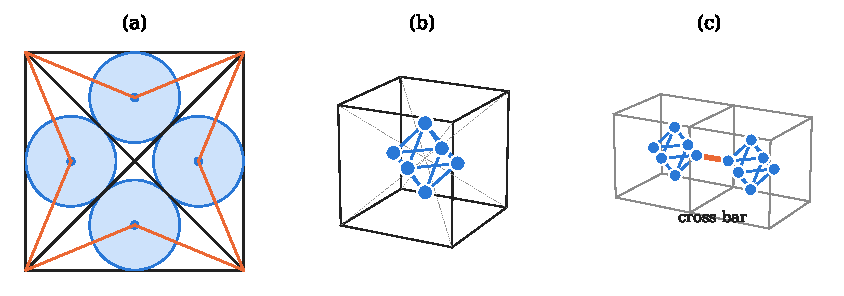
\includegraphics[width=\textwidth]{figures/fig1_construction.pdf}
\caption{(a) The planar construction: incentres of the four triangles cut by the diagonals, with balls of the inradius and lines to the corners. (b) In three dimensions the six incentres of the centre-to-face pyramids form an octahedron of edge $2R$. (c) Two cells of the framework: the cross-polytope bars inside each cell and one bridge between cells.}
\label{fig:construction}
\end{figure}

\section{The framework}\label{sec:construction}

Let $Q_n=[-1,1]^n$ and let $\e_1,\dots,\e_n$ be the standard basis. The pyramid over the facet $x_i=1$ is $\{x\in Q_n: x_i\ge |x_j|\ \forall j\}$, with base $x_i=1$ and walls $x_i=\pm x_j$. A point $t\e_i$ has distance $1-t$ to the base and $t/\sqrt2$ to every wall, so the incentre is $c\,\e_i$ with
\[
c=2-\sqrt2,\qquad R=1-c=\sqrt2-1,\qquad c\sqrt2=2R .
\]
The dots are $p_i^{s}=s\,c\,\e_i$ for $i=1,\dots,n$ and $s\in\{+1,-1\}$. Two dots on different axes are at distance $c\sqrt2=2R$, and $p_i^+$ is at distance $2-2c=2R$ from the dot $p_i^-+2\e_i$ of the next cell. All other distances are larger.

\begin{definition}
The \emph{bridged cross-polytope framework} $\mathcal F_n$ has the dots $p_i^s+2z$ ($z\in\Z^n$) as joints and a bar between every pair of touching balls: the $2n(n-1)$ \emph{intra bars} $\{p_i^s,p_j^t\}$, $i<j$, of each cell (the edges of the cross-polytope), and the $n$ \emph{bridges} $X_i=\{p_i^+,\ p_i^-+2\e_i\}$ per cell. Every bar has length $2R$. More generally, $\mathcal F_n(t)$ has the same graph with dots at $\pm t\e_i$, $0<t<1$.
\end{definition}

Per cell there are $2n$ joints, hence $2n^2$ degrees of freedom, and $2n^2-n$ bars; each ball touches $2n-1$ others. For Bloch displacements $\vu(p+2z)=\vu(p)\,e^{2i q\cdot z}$ write $z_i=e^{2iq_i}$. The rigidity matrix $R(q)$ has one row per bar; the row of a bar from joint $a$ to joint $b$ with unit direction $\hat d$ is $\vu\mapsto \hat d\cdot(\vu_b-\vu_a)$, with $\vu_b$ carrying the phase of its cell. A \emph{zero mode} is a vector in $\ker R(q)$ and a \emph{self-stress} a vector in $\ker R(q)^*$. By rank--nullity, the number of zero modes minus the number of self-stresses is $2n^2-(2n^2-n)=n$ at every $q$, the periodic Maxwell--Calladine count \cite{Maxwell1864,Calladine1978,Power2014}.

\section{Zero modes and self-stresses}\label{sec:counts}

Fix one cell. For displacements $\vu_i^s=\vu(p_i^s)$ write $\va_i=\tfrac12(\vu_i^++\vu_i^-)$ and $\vb_i=\tfrac12(\vu_i^+-\vu_i^-)$, and denote the $k$-th component of a vector by a superscript. For $i<j$ define
\[
\alpha_{ij}=a_i^i-a_j^i,\quad \beta_{ij}=a_i^j-a_j^j,\quad \kappa_{ij}=b_i^i+b_j^j,\quad \sigma_{ij}=b_i^j+b_j^i .
\]

\begin{lemma}\label{lem:block}
Under a homogeneous strain $\varepsilon$ plus displacements $\vu$, the first-order extension of the intra bar from $p_j^t$ to $p_i^s$ is
\begin{equation}\label{eq:ext}
\delta_{ij}^{st}=\tfrac{1}{\sqrt2}\Bigl[c(\varepsilon_{ii}+\varepsilon_{jj})+\kappa_{ij}+s\,\alpha_{ij}-t\,\beta_{ij}-st\,(2c\,\varepsilon_{ij}+\sigma_{ij})\Bigr].
\end{equation}
For a one-cell-periodic displacement the extension of the bridge $X_i$ is $2R\,\varepsilon_{ii}-2b_i^i$; for a Bloch displacement with $\varepsilon=0$ it is $\e_i\cdot(z_i\vu_i^--\vu_i^+)$.
\end{lemma}

\begin{proof}
The bar vector is $\ell=c(s\e_i-t\e_j)$, with unit vector $\ell/(c\sqrt2)$, and $\delta=\hat\ell\cdot(\varepsilon\ell+\vu_i^s-\vu_j^t)$. Expand with $\vu_i^s=\va_i+s\vb_i$ and $s^2=t^2=1$. For $X_i$ the bar vector is $2R\,\e_i$ and the displacement difference is $-2\vb_i$ in the periodic case.
\end{proof}

The functions $1,s,t,st$ on $\{\pm1\}^2$ are orthogonal. So the four bars between axes $i$ and $j$ impose the four scalar conditions $\kappa_{ij}=\alpha_{ij}=\beta_{ij}=\sigma_{ij}=0$ when $\varepsilon=0$, and
\begin{equation}\label{eq:sum}
\tfrac12\sum_{s,t}(\delta_{ij}^{st})^2=\bigl(c(\varepsilon_{ii}+\varepsilon_{jj})+\kappa_{ij}\bigr)^2+\alpha_{ij}^2+\beta_{ij}^2+\bigl(2c\,\varepsilon_{ij}+\sigma_{ij}\bigr)^2 .
\end{equation}
The linear problem splits into independent systems: one in the $n$ numbers $b_i^i$ (through $\kappa$), one in the $n^2$ entries of the $\va_i$ (through $\alpha,\beta$), and one in the $n(n-1)$ entries $b_i^j$, $i\ne j$ (through $\sigma$).

\begin{lemma}[cross-polytope]\label{lem:cross}
Let $n\ge3$. The cross-polytope (the intra bars of one cell) is infinitesimally rigid in $\R^n$ and has exactly $n(n-3)/2$ independent self-stresses. A basis: tension $w_{ij}$ on all four bars $\{p_i^\pm,p_j^\pm\}$, where $w=(w_{ij})_{i<j}$ satisfies $\sum_{j\ne i}w_{ij}=0$ for every $i$.
\end{lemma}

\begin{proof}
The conditions $\alpha_{ij}=\beta_{ij}=0$ say that for each $k$ all $a_j^k$ equal $a_k^k$, so $\va_j=\vv$ for all $j$; the map $\va\mapsto(\alpha,\beta)$ from $\R^{n^2}$ to $\R^{n(n-1)}$ has an $n$-dimensional kernel and is onto. Each $\sigma_{ij}$ involves $b_i^j,b_j^i$ only, so these $\binom n2$ conditions are independent and force the off-diagonal part of $B=(b_i^j)$ to be antisymmetric. The conditions $b_i^i+b_j^j=0$ form the system $x_i+x_j=0$ on the edges of $K_n$; for $n\ge3$ a triangle forces $x=0$. Its matrix, the unsigned incidence matrix of $K_n$, has rank $n$, and its left kernel (edge weights with $\sum_{j\ne i}w_{ij}=0$ at each vertex) has dimension $n(n-3)/2$. The kernel of the whole system is therefore $\vu_i^s=\vv+\Omega p_i^s$ with $\Omega$ antisymmetric, the trivial motions, and the number of self-stresses is $2n(n-1)-\bigl(2n^2-n(n+1)/2\bigr)=n(n-3)/2$. Expanding a stress on the four bars of a pair in the characters $1,s,t,st$, the $s$, $t$ and $st$ parts must vanish because the $\va$- and $\sigma$-systems have no relations, and the character-$1$ parts $w_{ij}$ must satisfy $\sum_{j\ne i}w_{ij}=0$.
\end{proof}

\begin{lemma}[periodic counts]\label{lem:bloch}
Let $n\ge3$. At a wavevector with no $q_i\in\pi\Z$, $\mathcal F_n(t)$ has exactly $n(n-1)/2$ zero modes per cell, the infinitesimal rotations of each cross-polytope with the common Bloch phase, and exactly $n(n-3)/2$ self-stresses, those of Lemma~\ref{lem:cross} with zero tension on the bridges. If exactly $k$ of the $q_i$ lie in $\pi\Z$ there are $n(n-1)/2+k$ zero modes and $n(n-3)/2+k$ self-stresses. At $q=0$ there are $n(n+1)/2$ zero modes and $n(n-1)/2$ self-stresses: for every $w\in\R^{\binom n2}$, tension $w_{ij}$ on the four bars $\{p_i^\pm,p_j^\pm\}$ and $\sqrt2\sum_{j\ne i}w_{ij}$ on $X_i$.
\end{lemma}

\begin{proof}
Intra rows carry no phase, so a zero mode restricts on each cell to $\vu_i^s=\vv+\Omega p_i^s$ with complex $\vv,\Omega$. Since $\e_i\cdot\Omega\e_i=0$, Lemma~\ref{lem:block} turns the bridge $X_i$ into $(z_i-1)v^i=0$: rotations survive at every phase and each $z_i=1$ frees one translation. The self-stress counts follow from rank--nullity, and the stated stresses balance every joint.
\end{proof}

\begin{remark}[credit and scope]
These counts use only the internal rigidity of the cross-polytope, the fact that a rotation moves each bridge end transversally, and rank--nullity; they are routine applications of the phase-periodic rigidity matrix \cite{Power2014} and of the rigid-unit analysis of linearly bridged frameworks \cite{Goodwin2006}. We record them because the explicit bases are used in Section~\ref{sec:elastic}. They use only bar directions, so they hold for $\mathcal F_n(t)$ for every $t\in(0,1)$, including the realization $t=\sqrt2-1$ of \cite[Section~7]{BorceaStreinu2021}. With a variable lattice the first-order count of the one-cell framework in three dimensions is $6$; for a periodicity lattice with $b$ body orbits the conditional Maxwell count is $(b+1)n(n-1)/2$, which gives the nine of \cite{BorceaStreinu2021} for $b=2$, $n=3$. For $n=2$ the square has one internal flex, and the counts are $2$ and $0$ at generic $q$, $3$ and $1$ at $q=0$. The numerical check (Section~\ref{sec:elastic}) confirms all counts for $n=2,\dots,8$.
\end{remark}

\section{Unit-spring elastic constants in every dimension}\label{sec:elastic}

\begin{theorem}\label{thm:elastic}
Let $n\ge3$. Give every bar of $\mathcal F_n$ unit spring constant, so that a bar extended by $\delta$ stores energy $\delta^2/2$, impose a homogeneous strain $\varepsilon$ and relax all joints. The energy per unit volume is
\begin{equation}\label{eq:W}
W(\varepsilon)=\frac{1}{2^{n}}\Bigl[\frac{2(n-1)^2}{n^2}\sum_i\varepsilon_{ii}^2+\frac{2}{n^2}\sum_{i\ne j}\varepsilon_{ii}\varepsilon_{jj}\Bigr],
\end{equation}
independent of the off-diagonal strains. With $W=\tfrac12 C_{ijkl}\varepsilon_{ij}\varepsilon_{kl}$,
\[
C_{11}=\frac{4(n-1)^2}{n^2\,2^n},\qquad C_{12}=\frac{4}{n^2\,2^n},\qquad \frac{C_{11}}{C_{12}}=(n-1)^2,
\]
every component of $C$ involving a shear strain vanishes, and the Poisson ratio for uniaxial stress along a cube axis is
\[
\nus=\frac{C_{12}}{C_{11}+(n-2)C_{12}}=\frac{1}{n^2-n-1}.
\]
\end{theorem}

The values of $\nus$ are $1/5,1/11,1/19,1/29,1/41$ for $n=3,\dots,7$ (Fig.~\ref{fig:modes}).

\begin{proof}
A homogeneous strain stretches the bars of every cell identically. In a Bloch decomposition of the relaxation over any periodic supercell only the $q=0$ component couples linearly to $\varepsilon$; the others add non-negative energy and are optimally zero. So it suffices to relax over one-cell-periodic displacements. By Lemma~\ref{lem:block} and \eqref{eq:sum} the energy per cell is
\[
\mathcal E=\sum_{i<j}\Bigl[\bigl(c(\varepsilon_{ii}+\varepsilon_{jj})+\kappa_{ij}\bigr)^2+\alpha_{ij}^2+\beta_{ij}^2+\bigl(2c\varepsilon_{ij}+\sigma_{ij}\bigr)^2\Bigr]+2\sum_i\bigl(R\,\varepsilon_{ii}-b_i^i\bigr)^2 .
\]
The variables $\va$ appear only in $\alpha,\beta$; take $\va=0$. The off-diagonal $b_i^j$ appear only in $\sigma_{ij}$, which can be chosen freely; take $\sigma_{ij}=-2c\,\varepsilon_{ij}$. This removes every off-diagonal strain, so all shear moduli vanish. (Each cross-polytope stays undeformed; shear is taken up by first-order rotations.)

With $e_i=\varepsilon_{ii}$, $x_i=b_i^i$ and $y_i=x_i+c\,e_i$, and using $c+R=1$,
\[
\mathcal E=\sum_{i<j}(y_i+y_j)^2+2\sum_i(e_i-y_i)^2 .
\]
The Hessian in $y$ is $2(nI+J)$, with $J$ the all-ones matrix, which is positive definite. Stationarity gives $n y_k+\sum_j y_j=2e_k$, hence $\sum_j y_j=\tfrac1n\sum_j e_j$ and $y_k=\tfrac1n\bigl(2e_k-\tfrac1n\sum_j e_j\bigr)$. The minimum of $y^TMy-2(2e)\cdot y+2|e|^2$ is $2|e|^2-2e\cdot y$, which evaluates to
\[
\mathcal E_{\min}=\frac{2(n-2)}{n}\sum_i e_i^2+\frac{2}{n^2}\Bigl(\sum_ie_i\Bigr)^2=\frac{2(n-1)^2}{n^2}\sum_ie_i^2+\frac{2}{n^2}\sum_{i\ne j}e_ie_j .
\]
Dividing by the cell volume $2^n$ gives \eqref{eq:W}. For uniaxial stress along $\e_1$, $\partial W/\partial e_j=0$ ($j\ge2$) reads $C_{12}e_1+(C_{11}+(n-2)C_{12})e_\perp=0$, and $C_{11}+(n-2)C_{12}=(4/n^22^n)\bigl((n-1)^2+n-2\bigr)$ gives $\nus=1/(n^2-n-1)$.
\end{proof}

\begin{remark}
(1) The proof does not use $n\ge3$, so \eqref{eq:W} also holds for $n=2$: $C_{11}=C_{12}=1/4$ and only the bulk modulus is non-zero. (2) For $\mathcal F_n(t)$ with unit springs on bars of unequal lengths the same computation applies with $t+(1-t)=1$ in place of $c+R=1$, and the formula is unchanged; the incentre $t=c$ is the unique $t$ at which all bars have the same length, so that ``unit springs'' means ``identical bars''. (3) The tensor is only positive semi-definite. The model has no angular stiffness or prestress, and $\nus$ is the response to stress along a cube axis, not an isotropic Poisson ratio or a property of a real compound.
\end{remark}

\emph{Prior art and check.} The formulas follow from minimizing spring energy; rigid-body kinematics alone does not give finite $C_{11}$ or $C_{12}$. We did not find $C_{11}/C_{12}=(n-1)^2$ or $\nus=1/(n^2-n-1)$ in Borcea and Streinu \cite[Section~7]{BorceaStreinu2021} or in the abstract of Goodwin \cite{Goodwin2006}; this bounded search is not evidence of priority, and the formulas may be immediate to specialists in periodic-framework elasticity. The script \texttt{results/rigidity-nd/rigidity\_nd.py} builds $R(q)$ and the relaxed elastic tensor from coordinates, without the decomposition, for $n=2,\dots,8$. It confirms every count at random $q$, at $q=0$ and on the planes $q_1=\dots=q_k=0$, that the stated bases span the self-stress spaces and the rotations span the generic zero modes, and the elastic constants to $10^{-12}$ with full relaxation, for $c=2-\sqrt2$ and for $c=0.3,0.75$. The script \texttt{proof\_steps.py} checks \eqref{eq:ext}, \eqref{eq:sum} and the minimization symbolically for $n=2,\dots,8$.

\begin{figure}[t]
\centering
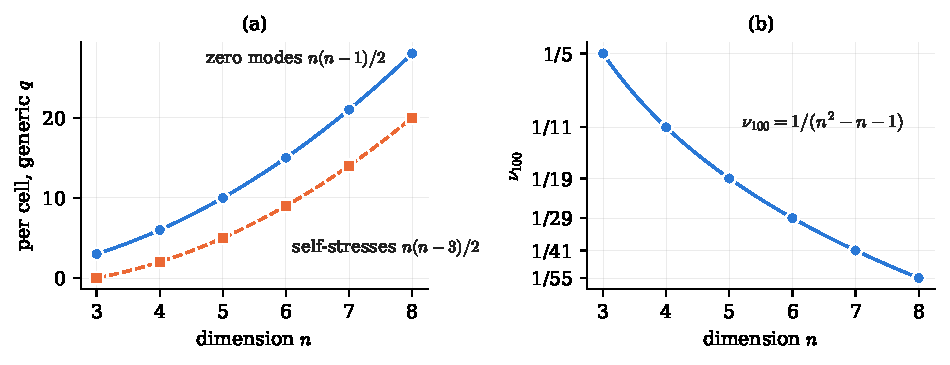
\includegraphics[width=0.92\textwidth]{figures/fig3_modes.pdf}
\caption{(a) Zero modes and self-stresses per cell at a generic wavevector (lines: Lemma~\ref{lem:bloch}; markers: rank of the numerically assembled rigidity matrix). (b) Poisson ratio $\nus$ with unit springs (line: Theorem~\ref{thm:elastic}; markers: full numerical relaxation).}
\label{fig:modes}
\end{figure}

\section{An exact motion from the cab framework to fcc}\label{sec:motion}

\subsection{The question}
Lemma~\ref{lem:bloch} and its variable-lattice analogue describe directions in which $\mathcal F_3$ can start to move. They do not say how far it can go. Here balls are joined centre to centre by bars of fixed length and must not overlap. Can the open framework, at packing fraction $\pi R^3=0.2233$, be moved continuously to a close packing?

This is not automatic. The natural symmetric motion, the $a^-a^-a^-$ tilt of the octahedra about $[111]$ \cite{Glazer1972} with the lattice kept cubic, locks at $60^\circ$ with packing fraction $27\pi\sqrt2/256=0.4686$ (Section~\ref{sec:supporting}). In corner-sharing ReO$_3$, by contrast, rotating the octahedra alone takes the anions to hexagonal close packing \cite{OKeeffeHyde1977,JohnssonLemmens2007}, which is observed under pressure at a rotation of $30^\circ$ \cite{Shan2026}. In the bridged framework the same tilt gives only $0.2637$ at $30^\circ$. Numerical searches with a free lattice found sampled paths to hcp and fcc, but greedy density ascent from other starting states jams between $0.58$ and $0.71$ (Section~\ref{sec:supporting}). We now give an exact motion.

\subsection{The curve}
Work in units of $K=2-\sqrt2$, in which the motif of one cell is
\[
P=\{\pm\e_1,\pm\e_2,\pm\e_3\},
\]
each ball has radius $1/\sqrt2$, and every bar has length $\sqrt2$. With row vectors and a lattice matrix $L$ whose rows $L_i$ are the periods, the centres are $p+nL$, $p\in P$, $n\in\Z^3$. The twelve octahedron edges join $\pm\e_i$ to $\pm\e_j$ ($i\ne j$), and the three bridges join $\e_i$ to $-\e_i+L_i$. Multiplying by $K$ and translating by $(1,1,1)$ gives the framework $\mathcal F_3$ of Section~\ref{sec:construction}, where $KL=2I$.

Write $\vb_i=L_i-2\e_i$ for the bridge vectors, so $L=2I+B$ with rows $\vb_i$. At the start, $\vb_i=\sqrt2\,\e_i$. Let
\[
C=\begin{pmatrix}0&-1&-1\\1&0&-1\\1&-1&0\end{pmatrix}.
\]
Its rows $C_i$ satisfy $C_i\cdot\e_i=0$ and $\norm{C_i}^2=2$. For $0\le s\le1$ put
\begin{equation}\label{eq:curve}
t=\frac{2s}{1+s^2},\qquad a=\frac{\sqrt2(1-s^2)}{1+s^2},\qquad \vb_i(s)=a\,\e_i+t\,C_i,\qquad L(s)=(2+a)I+tC .
\end{equation}
Then $a^2+2t^2=2$. With $\theta=2\arctan s$, $\vb_i=\sqrt2\bigl(\cos\theta\,\e_i+\sin\theta\,C_i/\sqrt2\bigr)$: each bridge turns through a right angle, at the same rate, in the plane spanned by its initial direction $\e_i$ and its final direction $C_i$, keeping length $\sqrt2$. The motif does not move. The endpoint is
\[
L(1)=2I+C=\begin{pmatrix}2&-1&-1\\1&2&-1\\1&-1&2\end{pmatrix}.
\]

\emph{Where $C$ comes from.} The integer matrix $L(1)$ is the exact fcc end state of a numerical path in the one-cell framework (Section~\ref{sec:supporting}): there the octahedron ends unrotated in its own frame, and the bridges are the rows of $C$. The curve \eqref{eq:curve} is the simplest motion that joins the two bridge configurations: each bridge rotates uniformly from $\sqrt2\,\e_i$ to $C_i$, which is possible with constant length because $C_i\perp\e_i$. That this rotation never makes two balls overlap is the content of Theorem~\ref{thm:motion}. Straight-line interpolation of the bridges would shorten them.

\begin{theorem}\label{thm:motion}
For $0\le s\le1$, the curve \eqref{eq:curve} is a smooth periodic motion of the three-dimensional bridged cross-polytope framework with the following properties.
\begin{enumerate}[label=(\alph*),leftmargin=2em]
\item Every bar has length $\sqrt2$, the lattice is nonsingular, and the octahedra keep their orientation.
\item No two balls overlap: all distinct centres are at least $\sqrt2$ apart. For $0\le s<1$ the only touching pairs are the $15$ bars per cell; at $s=1$ another $21$ contacts per cell appear at once, and each ball touches $12$ others.
\item The packing fraction $2\sqrt2\,\pi/\det L(s)$ increases strictly from $2\sqrt2\,\pi/(2+\sqrt2)^3=0.2233$ to $\pi/\sqrt{18}$, and $\det L$ falls from $(2+\sqrt2)^3$ to $12$.
\item At $s=1$ the centres form a translate of the fcc lattice.
\item For $0<s\le1$ the framework has space group $C2/m$, with point group $\{I,-I,m,-m\}$, where $m$ exchanges the second and third coordinates; the balls form two orbits, $\{\pm\e_1\}$ on the mirror and $\{\pm\e_2,\pm\e_3\}$ in general position. At $s=0$ the space group is $Pm\bar3m$.
\end{enumerate}
\end{theorem}

The motion is a deformation of the lattice, not a shear alone: the cell volume falls by a factor $(2+\sqrt2)^3/12=3.32$, and the packing fraction rises with it (Fig.~\ref{fig:motion}).

\begin{figure}[t]
\centering
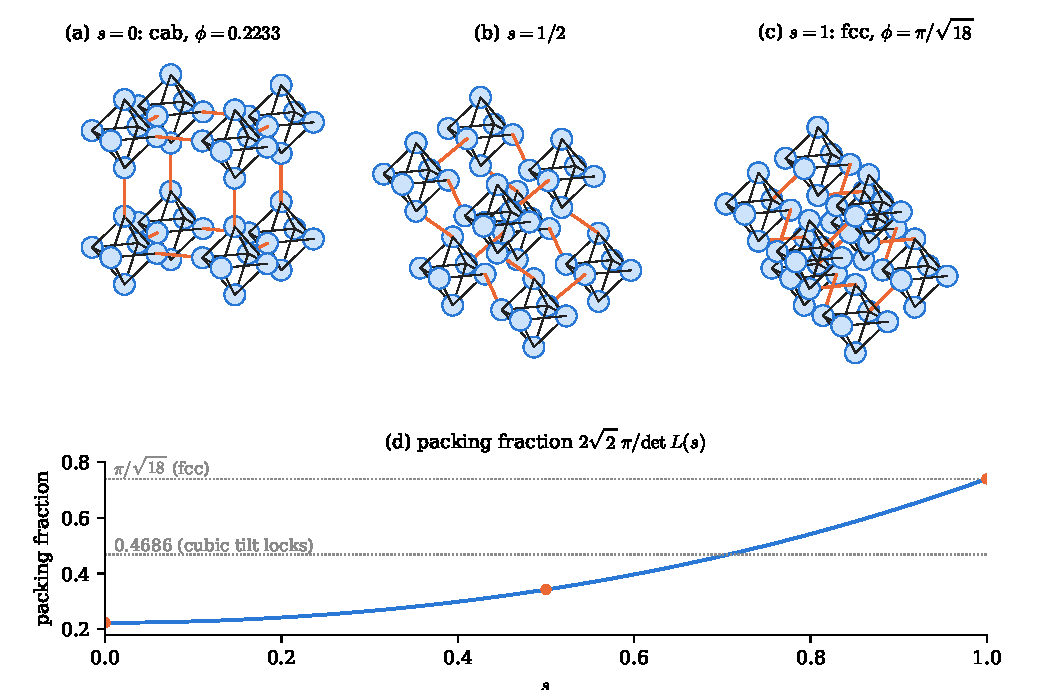
\includegraphics[width=\textwidth]{figures/fig_motion.pdf}
\caption{The motion of Theorem~\ref{thm:motion}, drawn from the exact formulas. (a)--(c) A block of $2\times2\times2$ cells at $s=0$, $1/2$, $1$, in the same orthographic view; balls are drawn at $0.42$ of their radius so that the bars show. Black: octahedron edges; orange: bridges. The octahedra keep their orientation while the lattice deforms. (d) Packing fraction along the motion; the dotted line at $0.4686$ is where the cubic-restricted tilt locks, a different path.}
\label{fig:motion}
\end{figure}

\subsection{Proof of (a), (c), (d), (e)}
The motif is fixed, so the twelve edges keep length $\sqrt2$, and $\norm{\vb_i}^2=a^2+2t^2=2$. Nonsingularity follows from the bound below. For (c), with $d=2+a$ and $a=\sqrt{2-2t^2}$, direct expansion gives $\det L=d^3+dt^2+2t^3$, and for $0<t<1$
\[
\frac{d}{dt}\det L=\frac{2t}{a}\bigl(-16-10a+3t^2+3at\bigr)<0,
\]
because the bracket is at most $-13-7a$. So $\det L$ decreases strictly between any two parameter values, and $t$ increases strictly with $s$. Each cell holds six balls of volume $(4\pi/3)2^{-3/2}$, which gives the packing fraction. For (d), the rows of $L(1)$ are integer vectors with even coordinate sum and $\det L(1)=12$, so $\Gamma=\Z^3L(1)$ has index $6$ in $D_3=\{z\in\Z^3:\sum z_i\text{ even}\}$, the fcc lattice of covolume $2$ \cite{ConwaySloane1999}. The six motif points have odd coordinate sum and lie in distinct cosets of $\Gamma$ (by (b) no two centres coincide), so they fill the odd coset of $D_3$, an fcc packing with minimum distance $\sqrt2$. For (e), $m$ commutes with $L(s)$ (it fixes $L_1$ and exchanges $L_2,L_3$), preserves $P$, and maps bridges to bridges ($\vb_1m=\vb_1$, $\vb_2m=\vb_3$). Any symmetry maps octahedra to octahedra, so its linear part is a signed permutation preserving the lattice $\Z^3L(s)$; for $0<s\le1$ only $\pm I$ and $\pm m$ do. The lattice has a basis $L_1$, $L_2$, $L_3=L_2m$ exchanged by the mirror, so it is centred monoclinic, and the group is $C2/m$.

\subsection{Proof of (b): a reduction to nine one-parameter inequalities}
Balls of one octahedron are at least $\sqrt2$ apart. For a nonzero integer row $n$ let $w=nL$ be the offset of another octahedron, and let $m_1\ge m_2\ge m_3$ be the absolute values of the coordinates of $w$, sorted. The squared distances between balls of the two octahedra are $\norm{w+v}^2$ with $v\in P-P=\{0,\pm2\e_i,\pm\e_i\pm\e_j\}$. Minimizing $2w\cdot v$ over each type of $v$, no two of these balls overlap if and only if
\begin{equation}\label{eq:ABC}
\text{(A)}\ \norm w^2-4m_1+2\ge0,\qquad \text{(B)}\ \norm w^2-2(m_1+m_2)\ge0,\qquad \text{(C)}\ \norm w^2\ge2 .
\end{equation}
These conditions are invariant under $n\mapsto-n$ and under the mirror $n\mapsto nm$, which exchanges two coordinates of $w$.

\begin{lemma}\label{lem:far}
For every $s\in[0,1]$ the smallest eigenvalue of $L(s)L(s)^T$ is at least $7/3$. Hence octahedra with $\norm n^2\ge5$ have all balls more than $\sqrt2$ apart.
\end{lemma}

\begin{proof}
Using $CC^T=I+J$, one finds $LL^T=(d^2+t^2)I+t^2J+dt\,E$, where $J$ is the all-ones matrix and $E$ has $E_{23}=E_{32}=-2$ and zeros elsewhere. In the orthonormal basis $\e_1$, $(\e_2+\e_3)/\sqrt2$, $(\e_2-\e_3)/\sqrt2$ it has the eigenvalue $(d+t)^2\ge4$ on the last vector, and on the first two the block with diagonal entries $\alpha=d^2+2t^2$, $\gamma=d^2+3t^2-2dt$ and off-diagonal entry $\sqrt2\,t^2$. With $d^2=6+4a-2t^2$, $\alpha-\tfrac73=\tfrac{11}3+4a$ and $\gamma-\tfrac73=\tfrac{11}3-4t+t^2+a(4-2t)\ge\tfrac23$ for $0\le t\le1$. So $(\alpha-\tfrac73)(\gamma-\tfrac73)\ge\tfrac{22}9>2\ge2t^4$, and the block minus $\tfrac73 I$ is positive semi-definite. If $\norm n^2\ge5$ then $\norm{nL}^2\ge\tfrac{35}3>6+4\sqrt2=(2+\sqrt2)^2$ (as $289>288$), and since $\norm v\le2$ every distance exceeds $\norm{nL}-2>\sqrt2$.
\end{proof}

If $\norm n^2=4$ then $n=\pm2\e_i$ and $\norm{nL}^2=4(d^2+2t^2)=4(6+4a)\ge24$. The remaining $26$ vectors with $1\le\norm n^2\le3$ form nine classes under sign and mirror. Table~\ref{tab:classes} lists, for each, the offset $w=dn+t\,nC$, its squared length, and the slack in (A) and (B), reduced with $a^2+2t^2=2$. Where the largest coordinate of $w$ depends on $s$, the slack is given for each candidate. Every entry is visibly non-negative for $0\le t\le1$, $a\ge0$, and (C) holds since $\norm w^2\ge6$ throughout. This proves non-overlap for all pairs and all $s$.

\begin{table}[t]
\caption{The nine classes of nearby octahedra (up to $n\mapsto-n$ and the mirror $m$), with $d=2+a$, $a^2+2t^2=2$. Slack is the left side of (A) or (B) in \eqref{eq:ABC}.}
\label{tab:classes}
\small
\begin{tabular}{@{}llll@{}}
\toprule
$n$ & $w=nL$ & slack in (A) & slack in (B)\\
\midrule
$\e_1$; $\e_2,\e_3$ & $(d,-t,-t)$; $(t,d,-t)$ & $0$ (bridge) & $2(1-t)+2a$\\
$(1,1,0)$ & $(d+t,d-t,-2t)$ & $2(1-t)^2+4+4a$ & $\ge2(1-t)^2+2+4a$\\
$(1,-1,0)$ & $(d-t,-d-t,0)$ & $2(1-t)(3+t)+4a$ & $4+4a-2t^2$\\
$(0,1,1)$ & $(2t,d-t,d-t)$ & $2(1-t)(7-t)+a(8-4t)$ & $2(1-t)(4-t)+a(6-4t)$\\
 & & or $2(1-t)^2+4+4a(1-t)$ & or $2(1-t)^2+2+4a(1-t)$\\
$(0,1,-1)$ & $(0,d+t,-d-t)$ & $2(d+t-1)^2$ & $2(d+t)(d+t-2)$\\
$(1,1,1)$ & $(d+2t,d-2t,d-2t)$ & $6(t-\tfrac43)^2+\tfrac43+a(8-4t)$ & $6(t-\tfrac23)^2+\tfrac{22}3+4a(2-t)$\\
$(1,-1,-1)$ & $(d-2t,-d,-d)$ & $2(1-t)(5+t)+2+a(8-4t)$ & $2(1-t)(5+t)+a(8-4t)$\\
$(1,1,-1)$ & $(d,d,-d-2t)$ & $12+8a-2t^2+4at$ & $10+8a-2t^2+4t+4at$\\
\bottomrule
\end{tabular}
\end{table}

\emph{Touching pairs.} A slack vanishes identically only for the bridges (class $\e_i$, condition (A)). Otherwise it vanishes only at $t=1$, $a=0$, that is $s=1$, in classes $\e_i$ (B), $(1,-1,0)$ (A), $(0,1,1)$ (A with $m_1=2t$, and B with $m_1+m_2=d+t$) and $(1,-1,-1)$ (B). These give the $21$ new contacts per cell of (b): at $s=1$ each ball goes from $5$ to $12$ contacts, all at once. The mirror class of $(1,-1,0)$ is $(1,0,-1)$, so at the end each octahedron touches the octahedra at offsets $\pm\e_i$, $\pm(1,-1,0)$, $\pm(1,0,-1)$, $\pm(0,1,1)$ and $\pm(1,-1,-1)$.

\emph{An independent exact certificate.} Before the reduction above was found, non-overlap was proved by computer \cite{RepoContinuous}: with the cruder bound $\norm{nL}\ge\norm n$ only the $171$ shifts with $\norm n^2\le11$ remain, giving $3248$ conditions $f_{n,v}(s)=(1+s^2)^2(\norm{nL(s)+v}^2-2)\ge0$, each a quartic in $s$ with coefficients in $\Q(\sqrt2)$. All $16{,}240$ coefficients in the degree-four Bernstein basis are non-negative, decided by exact rational comparisons; since the Bernstein basis functions are non-negative on $[0,1]$ \cite{Farouki2012}, this proves every inequality on the whole interval. Two separately written implementations agree, and $114$ coefficients are zero: five for each of the $18$ identically vanishing polynomials (the bars) and one for each of the $24$ polynomials that vanish at $s=1$, matching the contact count above. The written reduction is recorded with a symbolic check of every table entry in \texttt{results/fold-continuous-fcc/HAND-PROOF.md}.

\subsection{Context}
The motion is a statement about an ideal geometric model: bars of fixed length, hard balls, no energy, no angular stiffness. It says nothing about a transition in real CaB$_6$, whose connected octahedra are stiff \cite{LiRefsonDove2023}.

The closest community is the study of deformations of homogeneous sphere packings by Fischer, Koch and Sowa, in which sphere packings with free parameters are deformed with their contacts kept, and the $k/m/fn$ types are catalogued \cite{ITCSpherePackings,Fischer2004,KochFischerSowa2006}. In this language \textsf{cab} is the sphere-packing type $5/3/c3$. Sowa described ReO$_3$ under pressure by the deformation of a sphere packing formed by its oxygen anions \cite{Sowa1988}, Sowa and Ahsbahs studied the cooperative octahedral tilts of VF$_3$-type fluorides under pressure \cite{SowaAhsbahs1998}, and Sowa and Koch proposed a transition path between the diamond and lonsdaleite types \cite{SowaKoch2001}. In the ReO$_3$ and VF$_3$ cases the deformation rotates corner-sharing octahedra. The motion here differs in two ways: the octahedra are joined by bridges rather than shared corners and do not rotate, and the symmetry drops from $Pm\bar3m$ to $C2/m$ while the lattice deforms, ending at fcc rather than hcp. We have not read every paper in this literature, and a contact-preserving motion of the $5/3/c3$ packing to fcc may already be known there. We make no claim of priority. Periodic flexibility with a variable lattice has a general theory \cite{BorceaStreinu2010,MalesteinTheran2013}, and Borcea and Streinu's folding sketch \cite[Section~7]{BorceaStreinu2021} ends in a folded state of a different realization, not a packing. Ball packings with periodic constraints were studied by Connelly, Shen and Smith \cite{ConnellyShenSmith2014}; $\pi/\sqrt{18}$ is the maximum density of any sphere packing \cite{Hales2005}.

\section{Supporting results on finite motions}\label{sec:supporting}

In this section balls are joined centre to centre by bars of length $2R$ and may roll on each other.

\emph{The plane.} The 4.8.8 framework of squares and rods folds into the square tiling; this is the ``hinged squares with rods'' of Flores \cite{Flores}, who credits Stuart \cite{Stuart1963}, a relative of the rotating-squares mechanism \cite{GrimaEvans2000}. Alternate squares rotate by $\pm\theta$, the period is $L(\theta)=2R+2c\cos\theta$ in both directions, and $\nu=-1$ along the motion, as the criterion of \cite{Mitschke2013EPL} predicts. The closest non-bonded pair has gap $2\sqrt2\,c\cos(\theta+\pi/4)$, so a new contact appears at $\theta=\pi/4$, where the dots form a square lattice of spacing $2R$ and the packing fraction has risen from $\pi(\sqrt2-1)^2=0.5390$ to $\pi/4$. That no other pair comes closer first was checked numerically, not proved. These are elementary corollaries of a known mechanism.

\emph{The cubic-restricted tilt.} Rotate the octahedra of $\mathcal F_3$ alternately by $\pm\theta$ about $[111]$ and keep the lattice cubic. The bars fix the lattice parameter $a(\theta)=K_1+\sqrt{4R^2-2K_2^2}$, $K_2=\frac23c(1-\cos\theta)$, $K_1=2c\cos\theta+K_2$. At $\theta=60^\circ$, $a=8c/3$ exactly, each ball has six contacts and the packing fraction is $27\pi\sqrt2/256=0.4686$. This is a lock of the cubic path, not a jammed state: with a trigonal lattice, states up to $0.648$ are connected to $\theta=0$ on a grid. The six-contact net matches RCSR \textsf{sms} in the first ten terms of its coordination sequence; we did not check an isomorphism.

\emph{Sampled paths to close packing.} A numerical continuation (sequential linear programming with a deformable cell, in the manner of \cite{TorquatoJiao2010}, with bar equalities added) found a path of $793$ states in a $2\times2\times2$ supercell from the open state to hcp at $\pi/\sqrt{18}$; two layer slides extend it to pure fcc ($1193$ states). In the one-cell framework, free descent reached hcp ($333$ states), and a search steered toward a prescribed fcc end state reached it with density rising at every one of $268$ samples. Two checkers written within the project accept all four paths, with consecutive states at most $0.01$ apart and interpolated sub-states checked. This is sampled continuity, not a proof; the interpolated paths change bar lengths by up to $2\times10^{-5}$ of $2R$. Greedy density ascent from other starts jammed between $0.58$ and $0.71$, so the basin that reaches close packing is not generic for this method.

\emph{Exact end states.} The end states of these paths have exact integer closed forms (in units of $K$), checked in integer arithmetic: every bar exactly $2R$, no pair closer, $12$ contacts per ball, density exactly $\pi/\sqrt{18}$, and hcp or fcc by common-neighbour analysis. In the one-cell fcc end state the octahedron is unrotated in its own frame and the lattice is $L(1)$ of Section~\ref{sec:motion}; the hcp end state has lattice rows $\frac13(7,-1,4)$, $\frac13(-4,7,-1)$, $\frac13(-3,3,6)$. A certified continuous path to hcp remains open.

\section{A radius-ratio identity}\label{sec:ratio}

Let $P\subset\R^n$ be a convex polytope with the origin $O$ in its interior. For a facet $F$ let $\Pi_F=\operatorname{conv}(O\cup F)$, and for a ridge $E=F\cap G$ let $W_E$ be the hyperplane through $O$ and $E$ (the \emph{wall}). Suppose each $\Pi_F$ has an \emph{inscribed ball}, a ball in $\Pi_F$ tangent to every facet of $\Pi_F$, with centre $d_F$ (the \emph{dot}) and radius $r_F$.

\begin{lemma}\label{lem:unique}
If a convex polytope has a ball tangent to all its facet hyperplanes from inside, that ball is its unique largest inscribed ball.
\end{lemma}

\begin{proof}
Let the facets be $n_k\cdot x\le h_k$ with unit $n_k$ and the tangent ball $B(x,r)$, so $n_k\cdot x+r=h_k$. If $B(y,r')$ lies inside with $r'\ge r$, then $n_k\cdot(y-x)\le r-r'\le0$ for all $k$. Since the polytope is bounded there are $\lambda_k>0$ with $\sum\lambda_kn_k=0$, which forces $n_k\cdot(y-x)=0$ for all $k$ and $r'=r$; as the $n_k$ span $\R^n$, $y=x$.
\end{proof}

\begin{theorem}\label{thm:ratio}
Assume one of the following.
\begin{enumerate}[label=(H\arabic*),leftmargin=3em]
\item Every wall $W_E$ is a mirror of $P$, and $\Pi_F$ has an inscribed ball for one (hence every) facet.
\item $P$ has an insphere centred at $O$, and the angle $\varphi$ between the normals of any two adjacent facets is the same for all ridges.
\end{enumerate}
Then all dots have the same radius $r$ and the same distance $D$ from $O$; the balls of two facets sharing a ridge touch, at a point of the common wall; no two balls overlap; and the ball of radius $D-r$ centred at $O$ touches every ball. Consequently the hole/ball ratio is $(D-r)/r=2D/e-1$ with $e=2r$, the classical radius-ratio limit \cite{Pauling1929} of the polytope $Q$ of dots. Under (H1) $P$ is facet-transitive and $Q$ is vertex-transitive. Under (H2) $Q$ is a scaled polar dual of $P$, inscribed with all edges equal to $2r$, and $(D-r)/r=1/\sin(\varphi/2)-1$; conversely every convex inscribed polytope with equal edges and its circumcentre inside arises in this way.
\end{theorem}

\begin{proof}
\emph{(H1).} Let $\rho_E$ be the reflection in $W_E$. It fixes $O$ and $E$ pointwise and permutes the two facets through $E$. It cannot fix $F$: the plane of $F$ contains $E\subset W_E$ but not $O$, so if it were $\rho_E$-invariant it would be perpendicular to $W_E$ and $F$ would lie on both sides of $E$ in its plane. So $\rho_E(\Pi_F)=\Pi_G$, and by Lemma~\ref{lem:unique} $\rho_E(B_F)=B_G$. The ball $B_F$ is tangent to $W_E$ at a point fixed by $\rho_E$, so $B_F$ and $B_G$ touch there, with $r_F=r_G$ and $|Od_F|=|Od_G|$. The ridge graph is connected, so $r$ and $D$ are constant, and the reflections act transitively on facets. Balls lie in pyramids with disjoint interiors, so they do not overlap.

\emph{(H2).} Let $\varrho$ be the inradius and $\mathbf n_F$ the unit outer normal. As $O$ is equidistant from the planes of $F$ and $G$, $W_E$ is the internal bisector of the dihedral angle at $E$, with normal proportional to $\mathbf n_F-\mathbf n_G$, and the angle $\theta$ between $\mathbf n_F$ and $W_E$ has $\sin\theta=\sin(\varphi/2)$. The point $(\varrho-r)\mathbf n_F$ has distance $r$ from the base and $(\varrho-r)\sin(\varphi/2)$ from each wall; these agree for $r=\varrho\sin(\varphi/2)/(1+\sin(\varphi/2))$, so $D=\varrho-r=r/\sin(\varphi/2)$. The reflection in $W_E$ exchanges $d_F$ and $d_G$, at distance $2D\sin(\varphi/2)=2r$. The dots $D\mathbf n_F$ are a multiple of the vertices of the polar dual. Conversely, if $Q$ is inscribed with equal edges, its polar has all facets at one distance from $O$, and the angle between the normals at the ridge dual to an edge $qq'$ is $\angle qOq'$.
\end{proof}

\begin{remark}[scope]
(1) (H1) holds for the regular polytopes in every dimension, the rhombic dodecahedron, the $k$-gonal bipyramids of every height, and the Catalan duals of Wythoffian uniform polyhedra. On the rhombic dodecahedron the construction gives the equal-bond UB$_{12}$ boron net, RCSR \textsf{ubt}. (2) (H2) adds the duals of snub polyhedra and the tetragonal trapezohedron of the single shape dual to the uniform square antiprism. (3) Facet-transitivity and an insphere do not suffice: for tetragonal trapezohedra polar to square antiprisms of height $0.7$ and $1.3$ times the uniform one, every pyramid has an inscribed ball, but adjacent dots are $[1,1.017]\cdot2r$ and $[1,1.006]\cdot2r$ apart, so some contacts open. (4) The triangular prism with square sides is not facet-transitive; its pyramids have different inradii and the theorem does not apply. (5) The CN7 and CN9 polyhedra of the radius-ratio tables and the dodecahedral CN8 are not vertex-transitive, so (H1) cannot produce them; under (H2) the triangulated shapes would need to be inscribed equal-edged deltahedra, and the candidates $J_{13}$, $J_{84}$, $J_{51}$ are not inscribed. The construction explains one structural limit of the radius-ratio rule; it does not address the softness and size effects behind most of its failures \cite{George2020}. The script \texttt{results/radius-ratio/radius\_ratio.py} checks the conclusion on $20$ polytopes (Table~\ref{tab:ratio}) and the four counterexamples.
\end{remark}

\begin{table}[t]
\caption{Hole/ball ratio of the incentre construction (inscribed balls by linear programming) against the classical radius-ratio limit of $Q$. All rows satisfy (H1) except the last two, which satisfy (H2).}
\label{tab:ratio}
\begin{tabular}{llcc}
\toprule
$P$ & $Q$ (coordination) & hole/ball & classical \\
\midrule
tetrahedron & tetrahedron (CN4) & 0.2247 & $\sqrt{3/2}-1=0.2247$\\
cube & octahedron (CN6) & 0.4142 & $\sqrt2-1=0.4142$\\
octahedron & cube (CN8) & 0.7321 & $\sqrt3-1=0.7321$\\
dodecahedron & icosahedron (CN12) & 0.9021 & 0.9021\\
rhombic dodecahedron & cuboctahedron (CN12) & 1.0000 & 1\\
triangular bipyramid, any height & trigonal prism (CN6) & 0.5275 & 0.5275\\
icosahedron & dodecahedron (CN20) & 1.8025 & 1.8025\\
tesseract & 16-cell (4D) & 0.4142 & 0.4142\\
\midrule
pentagonal icositetrahedron & snub cube & 1.6874 & 1.6874\\
trapezohedron (one shape) & square antiprism (CN8) & 0.6453 & 0.6453\\
\bottomrule
\end{tabular}
\end{table}

\section{The CaB$_6$ packing maximum}\label{sec:cab6}

Tiled by the cubic lattice, the dots of the cube are the boron positions of the equal-bond model of CaB$_6$ \cite{PaulingWeinbaum1934}: Ca at $1a$ $(0,0,0)$, B at $6f$ $(x,\tfrac12,\tfrac12)$ and permutations, $x=(\sqrt2-1)/2$. Consider hard spheres of radius $r_{\rm L}$ on the Ca sites and $r_{\rm S}$ on the B sites, with $x$ and the lattice parameter $a$ free, and $\gamma=r_{\rm S}/r_{\rm L}$.

\begin{theorem}\label{thm:cab6}
The maximal packing fraction of the CaB$_6$ structure type at size ratio $\gamma$ is
\[
\phi_{\max}(\gamma)=\begin{cases}\dfrac{\pi}{6}\bigl(1+6\gamma^3\bigr), & 0<\gamma\le\sqrt2-1,\\[2mm]
\dfrac{\pi}{6}(\sqrt2-1)^3\bigl(6+\gamma^{-3}\bigr), & \gamma\ge\sqrt2-1.\end{cases}
\]
Its global maximum is $\phi^*=\frac{\pi}{6}(30\sqrt2-41)=0.746865$, attained only at $\gamma=\sqrt2-1$, $x=(\sqrt2-1)/2$, $a=2r_{\rm L}$. There the Ca spheres touch each other and each B sphere touches five B spheres, but Ca and B do not touch: $d_{\rm Ca\text{-}B}=0.73681\,a>r_{\rm L}+r_{\rm S}=0.70711\,a$. Moreover $\phi_{\max}(\gamma)>\pi/(3\sqrt2)$ (fcc) exactly when $\bigl(\tfrac{\sqrt2-1}{6}\bigr)^{1/3}=0.41023<\gamma<(4+7\sqrt2)^{-1/3}=0.41591$.
\end{theorem}

\begin{proof}
Set $a=1$; then $\phi=\frac{4\pi}{3}(r_{\rm L}^3+6r_{\rm S}^3)$. Three of the constraints are Ca--Ca, $2r_{\rm L}\le1$; B--B inside an octahedron, $2r_{\rm S}\le\sqrt2(\tfrac12-x)$; and B--B between octahedra, $2r_{\rm S}\le2x$. The last two give $r_{\rm S}\le\min\bigl((\tfrac12-x)/\sqrt2,\,x\bigr)\le m^*=(\sqrt2-1)/2$, with equality only at $x^*=(\sqrt2-1)/2$. Hence $\phi\le\frac{\pi}{6}(1+6\gamma^3)$ from $r_{\rm L}\le\frac12$, and $\phi\le\frac{4\pi}{3}m^{*3}(6+\gamma^{-3})$ from $r_{\rm S}\le m^*$; the first bound is smaller for $\gamma\le\sqrt2-1$. Both are attained at $x=x^*$, with $r_{\rm L}=\frac12$, $r_{\rm S}=\gamma/2$ or $r_{\rm S}=m^*$, $r_{\rm L}=m^*/\gamma$, provided no other pair of spheres overlaps. That remaining step is proved by classifying every pair of sites and every lattice translation; the exact minimum distances are $d_{\rm CaCa}=1$, $d_{\rm CaB}=\sqrt{x^2+\tfrac12}$ and $d_{\rm BB}=\min\bigl(\sqrt2(\tfrac12-x),2x\bigr)$, and $r_{\rm L}+r_{\rm S}\le0.70711<0.73681$ throughout \cite{RepoCab6}. The window follows from $6\gamma^3>\sqrt2-1$ and $\gamma^{-3}>4+7\sqrt2$.
\end{proof}

\begin{remark}
(1) The curve was plotted, for this and 23 other lattices, by Horst and Travesset \cite[Fig.~3]{HorstTravesset2016}, and the peak position can be read from their figure. The location $\gamma=\sqrt2-1$ may also be stated by Travesset \cite{Travesset2017}, which we could not read; we did not find the closed form in the sources we read, and we do not claim it is new. (2) The maximum is a cusp (Fig.~\ref{fig:cab6}), and the window above fcc is narrow and asymmetric, $-0.0040$ and $+0.0017$ about $\sqrt2-1$. (3) CaB$_6$ is not a densest binary packing at this size ratio: the NaCl type reaches $\pi(5-3\sqrt2)/3=0.7931$, and CaB$_6$ is absent from the densest binary packings of \cite{Hopkins2012} and from the Murray--Sanders list of structures beating fcc \cite{MurraySanders1980}. CaB$_6$-type nanoparticle superlattices are observed \cite{Shevchenko2006}.
\end{remark}

\begin{figure}[t]
\centering
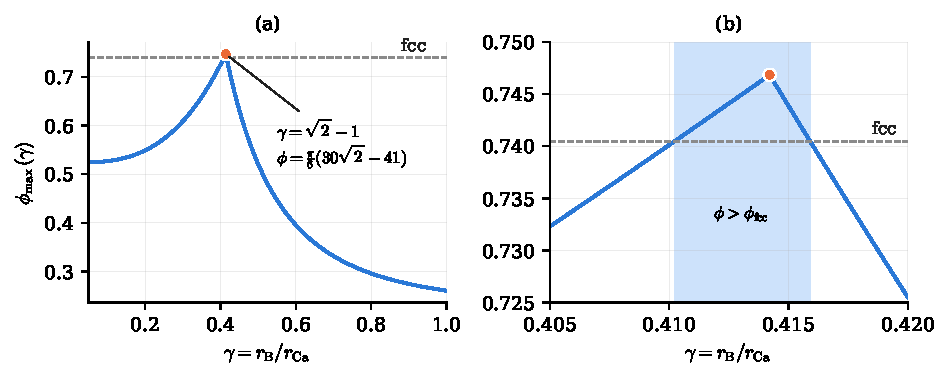
\includegraphics[width=0.92\textwidth]{figures/fig4_cab6.pdf}
\caption{(a) Maximal packing fraction of the CaB$_6$ type versus size ratio (Theorem~\ref{thm:cab6}); dashed line: fcc. (b) Detail of the cusp; shaded: the window where it exceeds fcc.}
\label{fig:cab6}
\end{figure}

\section{Open questions}

Whether the elastic formulas of Theorem~\ref{thm:elastic} are already in the periodic-framework elasticity literature, and whether a contact-preserving motion of the $5/3/c3$ packing to fcc is known in the sphere-packing deformation literature, are the two questions we most want answered by specialists. Mathematically open are a certified continuous path to hcp, a description of the set of close-packed states reachable from the open framework and how they connect, analogous motions in dimensions $n\ge4$, and the behaviour of these frameworks with angular stiffness. All results here have had internal review only; none has had independent human review.

\section*{Acknowledgments}
The drawing began as a doodle the author made on the backs of tests and on napkins, because the pattern was satisfying.

AI assistance: most of the computation, proofs, checking and writing were done by AI models under the author's direction. Claude models from Anthropic (Claude Opus 5.5 and other Claude models) drafted proofs, code and text, ran the literature searches and the numerical searches for fold paths, and wrote the symmetry-reduced proof of Theorem~\ref{thm:motion}(b) for this version. Some contributions were developed with OpenAI Codex and GPT models: GPT-6 (Codex) derived the explicit curve of Section~\ref{sec:motion}, its first written proof and the first exact certificate, and prepared the all-pairs attainment proof for Theorem~\ref{thm:cab6}; GPT-6.1 Sol independently checked the analytic reductions and supplied a second exact implementation; a research assessment prepared with Codex (GPT-6) shaped the priorities of this version. All reviews so far were performed by AI models under direction; no person other than the author has checked the proofs. Responsibility for the content rests with the author.

\section*{Code availability}
{\sloppy Every number in this paper is reproduced by the scripts in the repository \url{https://github.com/aska-digital/incentre-lattice}, where each result has a folder under \texttt{results/} with a written proof (\texttt{PROOF.md}), a deterministic verifier and a certificate; \texttt{make verify} replays all of them. The results of v1 are archived in release v1.0.0, doi:\href{https://doi.org/10.5281/zenodo.23322080}{10.5281/zenodo.23322080}; the additions of this version (\texttt{results/fold-continuous-fcc}, \texttt{results/cab6-packing/ATTAINMENT.md}) will be archived with the release of this version under the concept DOI \href{https://doi.org/10.5281/zenodo.23322079}{10.5281/zenodo.23322079}. Figure~\ref{fig:motion} is generated from the exact formulas by \texttt{papers/source/figures/make\_fold\_figure.py}.\par}

\bibliographystyle{amsplain}
\bibliography{refs}

\end{document}
